\documentclass{article} \usepackage[preprint]{nips_2018}

\usepackage{times}





\usepackage{natbib}
\usepackage[utf8]{inputenc} \usepackage[T1]{fontenc}    \usepackage{hyperref}       \usepackage{url}            \usepackage{booktabs}       \usepackage{graphicx}
\usepackage{wrapfig,lipsum,booktabs}
\usepackage{subcaption}
\usepackage{amsmath}
\usepackage{tikz}
\usepackage{graphicx}
\usetikzlibrary{positioning}


\newcommand\loss{L}
\newcommand\hood{\mathcal{S}}
\newcommand{\adv}{\ensuremath{\text{adv}}}
\newcommand{\D}{\mathcal{D}}
\newcommand{\E}{\mathbb{E}}
\newcommand{\R}{\mathbb{R}}
\usepackage{amsfonts}
\usepackage{mathtools}
\usepackage{framed}
\usepackage{microtype}
\setcounter{bottomnumber}{1}


\newcommand{\reals}{\mathbb{R}}
\newcommand{\subjectto}{{\text {subject to}}}
\DeclareMathOperator*{\argmin}{\arg\!\min}
\DeclareMathOperator*{\expectation}{\mathbb{E}}
\DeclareMathOperator*{\argmax}{\arg\!\max}
\DeclareMathOperator*{\softmin}{\mathrm{soft}\!\min}
\DeclareMathOperator*{\infsup}{\inf\!/\!\sup}
\newcommand\myeq{\stackrel{\left(\lambda\right)}{\inf\!\sup}}
\newcommand{\advgrad}{\overset{\left(adv\right)}{\nabla}}
\newcommand\Myperm[2][n]{\prescript{#1\mkern-2.5mu}{}P_{#2}}
\newcommand{\widesim}[2][1.5]{
  \mathrel{\overset{#2}{\scalebox{#1}[1]{}}}
}

\usepackage{epsfig}
\usepackage{url}

\usepackage{lipsum}

\newcommand\blfootnote[1]{\begingroup
  \renewcommand\thefootnote{}\footnote{#1}\addtocounter{footnote}{-1}\endgroup
}



\usepackage{siunitx}
\usepackage{algorithm,algpseudocode}
\usepackage{xr-hyper}
\usepackage{xr}
\usepackage{xr}
\usepackage{wrapfig}
\usepackage{amsmath,amsthm}
\usepackage{amssymb}
\usepackage{epstopdf}
\usepackage{mathtools}

\newcommand{\manifoldmixup}{\textit{Manifold Mixup}}
\newcommand{\inputmixup}{Input Mixup}

\renewcommand\epsilon\varepsilon


\title{Manifold Mixup: Better Representations by Interpolating Hidden States}


\author{
  Vikas Verma*   \\
  Aalto Univeristy, Finland \hfill\\
  \texttt{vikas.verma@aalto.fi} \\
   \And
   Alex Lamb* \\
   Montr\'{e}al Institute for Learning Algorithms \\
   \texttt{lambalex@iro.umontreal.ca} \\
   \And
   Christopher Beckham \\
   Montr\'{e}al Institute for Learning Algorithms \\
   \texttt{christopher.j.beckham@gmail.com} \\
      \And
   Amir Najafi \hspace{1.4cm} \\
   Sharif University of Technology\hspace{1.4cm}  \\
   \texttt{najafy@ce.sharif.edu}\hspace{1.4cm} \\
   \AND
   Ioannis Mitliagkas \\
   Montr\'{e}al Institute for Learning Algorithms \\
   \texttt{imitliagkas@gmail.com} \\
   \And
   Aaron Courville\hspace{0.8cm} \\
   Montr\'{e}al Institute for Learning Algorithms \\
   \texttt{courvila@iro.umontreal.ca} \\
   \AND
   \hspace{0.8cm}David Lopez-Paz\\
   \hspace{0.8cm}Facebook AI Research\\
   \hspace{0.8cm}\texttt{dlp@fb.com} \\
   \And
   \hspace{0.5cm}Yoshua Bengio \\
   \hspace{0.5cm}Montr\'{e}al Institute for Learning Algorithms \\
   \hspace{0.5cm}CIFAR Senior Fellow \\
   \hspace{0.5cm}\texttt{yoshua.umontreal@gmail.com} \\
}



\renewcommand\epsilon\varepsilon
\newcommand{\fix}{\marginpar{FIX}}
\newcommand{\new}{\marginpar{NEW}}

\begin{document}

\newtheorem{thm}{Theorem}[section]
\newtheorem{thm2}{Theorem}
\newtheorem{corl}{Corollary}
\newtheorem{note}[thm2]{Note}
\newtheorem{lemma}{Lemma}
\newtheorem{definition}{Definition}
\newtheorem{remark}{Remark}
\newtheorem{claim}{Claim}

\maketitle



\begin{abstract}


Deep neural networks excel at learning the training data, but often provide incorrect and confident predictions when evaluated on slightly different test examples.
This includes distribution shifts, outliers, and adversarial examples.
To address these issues, we propose \manifoldmixup{}, a simple regularizer that encourages neural networks to predict less confidently on interpolations of hidden representations.
\manifoldmixup{} leverages semantic interpolations as additional training signal, obtaining neural networks with smoother decision boundaries at multiple levels of representation. 
As a result, neural networks trained with \manifoldmixup{} learn class-representations with fewer directions of variance.
We prove theory on why this flattening happens under ideal conditions, validate it on practical situations, and connect it to previous works on information theory and generalization.
In spite of incurring no significant computation and being implemented in a few lines of code, \manifoldmixup{} improves strong baselines in supervised learning, robustness to single-step adversarial attacks, and test log-likelihood.
\end{abstract}

\section{Introduction}

Deep neural networks are the backbone of state-of-the-art systems for computer vision, speech recognition, and language translation \citep{lecun2015deep}.  
However, these systems perform well only when evaluated on instances very similar to those from the training set.  
When evaluated on slightly different distributions, neural networks often provide incorrect predictions with strikingly high confidence.
This is a worrying prospect, since deep learning systems are being deployed in settings where data may be subject to distributional shifts. 
Adversarial examples \citep{szegedy2013adv} are one such failure case: deep neural networks with nearly perfect performance provide incorrect predictions with very high confidence when evaluated on perturbations imperceptible to the human eye.
Adversarial examples are a serious hazard when deploying machine learning systems in security-sensitive applications.
More generally, deep learning systems quickly degrade in performance as the distributions of training and testing data differ slightly from each other \citep{ben2010theory}.

\begin{figure*}[t!]
        \centering
        \begin{subfigure}{0.30\textwidth}
            \centering
            \includegraphics[scale=0.45]{figures/2d_analytical/vanilla_spiral.png}
            \caption[]{}    
        \end{subfigure}
\begin{subfigure}{0.30\textwidth}  
            \centering 
            \includegraphics[scale=0.45]{figures/2d_analytical/mm_spiral.png}
            \caption[]{}    
        \end{subfigure}
        \begin{subfigure}{0.30\textwidth}  
            \centering 
            \includegraphics[scale=0.45]{figures/2d_analytical/svdplots_layer1.png}
            \caption[]{}    
        \end{subfigure}
        \begin{subfigure}[b]{0.30\textwidth}   
            \centering 
            \includegraphics[scale=0.45]{figures/2d_analytical/vanilla_hidden.png}
            \caption[]{}    
        \end{subfigure}
\begin{subfigure}[b]{0.30\textwidth}   
            \centering 
            \includegraphics[scale=0.45]{figures/2d_analytical/mm_hidden.png}
            \caption[]{}    
        \end{subfigure}
        \begin{subfigure}[b]{0.30\textwidth}  
            \centering 
            \includegraphics[scale=0.45]{figures/2d_analytical/svdplots_layer3.png}
            \caption[]{}    
        \end{subfigure}
        
        \caption{An experiment on a network trained on the 2D spiral dataset with a 2D bottleneck hidden representation in the middle of the network. Manifold mixup has three effects on learning when compared to vanilla training. First, it smoothens decision boundaries (from a. to b.). Second, it improves the arrangement of hidden representations and encourages broader regions of low-confidence predictions (from d. to e.). Black dots are the hidden representation of the inputs sampled uniformly from the range of the input space.  Third, it flattens the representations (c. at layer 1, f. at layer 3). Figure \ref{appendix:figure:variousregs} shows that these effects are not accomplished by other well-studied regularizers (input mixup, weight decay, dropout, batch normalization, and adding noise to the hidden representations).}
        \label{fig:2dbottleneck}
\end{figure*}

\iffalse
\begin{figure*}[t!]
  \centering
  \includegraphics[width=\linewidth]{figures/2d_analytical/mm_new_figure_1_a.png}
  \caption{An experiment on a network trained on the 2D spiral dataset with a 2D bottleneck hidden representation in the middle of the network. Manifold mixup has three effects on learning when compared to vanilla training. First, it smoothens decision boundaries (from a. to b.). Second, it improves the arrangement of hidden representations and encourages broader regions of low-confidence predictions (from d. to e.).  Third, it flattens the representations (c. at layer 1, f. at layer 3). Figure \ref{appendix:figure:variousregs} shows that these effects are not accomplished by other well-studied regularizers (input mixup, weight decay, dropout, batch normalization, and adding noise to the hidden representations).}
  \label{fig:2dbottleneck}
\end{figure*}
\fi

In this paper, we realize several troubling properties concerning the hidden representations and decision boundaries of state-of-the-art neural networks.
First, we observe that the decision boundary is often sharp and close to the data.
Second, we observe that the vast majority of the hidden representation space corresponds to high confidence predictions, both on and off of the data manifold.

Motivated by these intuitions we propose \manifoldmixup{} (Section~\ref{sec:manifold_mixup}), a simple regularizer that addresses several of these flaws by training neural networks on linear combinations of hidden representations of training examples. 
Previous work, including the study of analogies through word embeddings (e.g. king  man  woman  queen), has shown that interpolations are an effective way of combining factors \citep{mikolov2013wordembed}.  
Since high-level representations are often low-dimensional and useful to linear classifiers, linear interpolations of hidden representations should explore meaningful regions of the feature space effectively.
To use combinations of hidden representations of data as novel training signal, we also perform the same linear interpolation in the associated pair of one-hot labels, leading to mixed examples with soft targets.

To start off with the right intuitions, Figure~\ref{fig:2dbottleneck} illustrates the impact of \manifoldmixup{} on a simple two-dimensional classification task with small data.
In this example, vanilla training of a deep neural network leads to an irregular decision boundary (Figure~\ref{fig:2dbottleneck}a), and a complex arrangement of hidden representations (Figure~\ref{fig:2dbottleneck}d).
Moreover, every point in both the raw (Figure~\ref{fig:2dbottleneck}a) and hidden (Figure~\ref{fig:2dbottleneck}d) data representations is assigned a prediction with very high confidence.
This includes points (depicted in black) that correspond to inputs off the data manifold!  
In contrast, training the same deep neural network with \manifoldmixup{} leads to a smoother decision boundary (Figure~\ref{fig:2dbottleneck}b) and a simpler (linear) arrangement of hidden representations (Figure~\ref{fig:2dbottleneck}e).
In sum, the representations obtained by \manifoldmixup{} have two desirable properties: the class-representations are flattened into a minimal amount of directions of variation, and all points in-between these flat representations, most unobserved during training and off the data manifold, are assigned low-confidence predictions.
 
This example conveys the central message of this paper:
\begin{center}
    \emph{Manifold Mixup improves the hidden representations and decision boundaries of neural networks at multiple layers.}
\end{center}


\begin{figure*}[t]
\centering
\begin{minipage}{0.17\textwidth}
\begin{tikzpicture}
  \node (img)  {\includegraphics[scale=0.25]{figures/2d_analytical/wd_spiral.png}};
    \node[left=of img, node distance=0cm, rotate=90, anchor=center,yshift=-0.7cm] {Input Space};
    \node[left=of img, node distance=0cm, rotate=90, anchor=center,yshift=-0.7cm,font=\color{red}] {};
 \end{tikzpicture}
\end{minipage}\begin{minipage}{0.17\textwidth}
\begin{tikzpicture}
  \node (img)  {\includegraphics[scale=0.25]{figures/2d_analytical/noise_spiral.png}};
  \node[left=of img, node distance=0cm, rotate=90, anchor=center,yshift=-0.7cm,font=\color{red}] {};
\end{tikzpicture}
\end{minipage}\begin{minipage}{0.17\textwidth}
\begin{tikzpicture}
  \node (img)  {\includegraphics[scale=0.25]{figures/2d_analytical/dropout_spiral.png}};
  \node[left=of img, node distance=0cm, rotate=90, anchor=center,yshift=-0.7cm,font=\color{red}] {};
\end{tikzpicture}
\end{minipage}\begin{minipage}{0.17\textwidth}
\begin{tikzpicture}
  \node (img)  {\includegraphics[scale=0.25]{figures/2d_analytical/bn_spiral.png}};
  \node[left=of img, node distance=0cm, rotate=90, anchor=center,yshift=-0.7cm,font=\color{red}] {};
\end{tikzpicture}
\end{minipage}\begin{minipage}{0.17\textwidth}
\begin{tikzpicture}
  \node (img)  {\includegraphics[scale=0.25]{figures/2d_analytical/mixup_spiral.png}};
  \node[left=of img, node distance=0cm, rotate=90, anchor=center,yshift=-0.7cm,font=\color{red}] {};
\end{tikzpicture}
\end{minipage}

\begin{minipage}{0.17\textwidth}
\begin{tikzpicture}
  \node (img)  {\includegraphics[scale=0.25]{figures/2d_analytical/wd_hidden.png}};
  \node[below=of img, node distance=0cm, yshift=1cm] {Weight Decay};
  \node[left=of img, node distance=0cm, rotate=90, anchor=center,yshift=-0.7cm] {Hidden space};
 \end{tikzpicture}
\end{minipage}\begin{minipage}{0.17\textwidth}
\begin{tikzpicture}
  \node (img)  {\includegraphics[scale=0.25]{figures/2d_analytical/noise_hidden.png}};
  \node[below=of img, node distance=0cm, yshift=1cm] {Noise};
  \node[left=of img, node distance=0cm, rotate=90, anchor=center,yshift=-0.7cm] {};
\end{tikzpicture}
\end{minipage}\begin{minipage}{0.17\textwidth}
\begin{tikzpicture}
  \node (img)  {\includegraphics[scale=0.25]{figures/2d_analytical/dropout_hidden.png}};
  \node[below=of img, node distance=0cm, yshift=1cm] {Dropout};
  \node[left=of img, node distance=0cm, rotate=90, anchor=center,yshift=-0.7cm] {};
\end{tikzpicture}
\end{minipage}\begin{minipage}{0.17\textwidth}
\begin{tikzpicture}
  \node (img)  {\includegraphics[scale=0.25]{figures/2d_analytical/bn_hidden.png}};
  \node[below=of img, node distance=0cm, yshift=1cm] {Batch-Norm};
  \node[left=of img, node distance=0cm, rotate=90, anchor=center,yshift=-0.7cm] {};
\end{tikzpicture}
\end{minipage}\begin{minipage}{0.17\textwidth}
\begin{tikzpicture}
  \node (img)  {\includegraphics[scale=0.25]{figures/2d_analytical/mixup_hidden.png}};
  \node[below=of img, node distance=0cm, yshift=1cm] {Input Mixup};
  \node[left=of img, node distance=0cm, rotate=90, anchor=center,yshift=-0.7cm] {};
\end{tikzpicture}
\end{minipage}\caption{The same experimental setup as Figure~\ref{fig:2dbottleneck}, but using a variety of competitive regularizers.  This shows that the effect of concentrating the hidden representation for each class and providing a broad region of low confidence between the regions is not accomplished by the other regularizers (although input space mixup does produce regions of low confidence, it does not flatten the class-specific state distribution).  Noise refers to gaussian noise in the input layer, dropout refers to dropout of 50\% in all layers except the bottleneck itself (due to its low dimensionality), and batch normalization refers to batch normalization in all layers.  }
\label{appendix:figure:variousregs}
\end{figure*}


More specifically, \manifoldmixup{} improves generalization in deep neural networks because it:
\begin{itemize}
    \item Leads to smoother decision boundaries that are further away from the training data, at multiple levels of representation.  Smoothness and margin are well-established factors of generalization \citep{bartlett1998generalization,lee1995vcsmooth}.  

    \item Leverages interpolations in deeper hidden layers, which capture higher level information \citep{zeiler2013visual} to provide additional training signal.

    \item Flattens the class-representations, reducing their number of directions with significant variance (Section~\ref{sec:flatten}). This can be seen as a form of compression, which is linked to generalization by a well-established theory \citep{tishby2015info,shwartz2017info} and extensive experimentation \citep{alemi2016bottleneck,belghazi2018mine,goyal2018transfer,achille2018information}.
\end{itemize}

Throughout a variety of experiments, we demonstrate four benefits of \manifoldmixup{}:

\begin{itemize}
    \item Better generalization than other competitive regularizers (such as Cutout, Mixup, AdaMix, and Dropout) (Section~\ref{sec:supervised}).

    \item Improved log-likelihood on test samples (Section~\ref{sec:supervised}).
    


    \item Increased performance at predicting data subject to novel deformations (Section~\ref{sec:deformations}).

    \item Improved robustness to single-step adversarial attacks.  This is the evidence  that \manifoldmixup{} pushes the decision boundary away from the data in some directions (Section~\ref{sec:adversarial}). This is not to be confused with full adversarial robustness, which is defined in terms of moving the decision boundary away from the data in \emph{all} directions.
\end{itemize}










\iffalse
\begin{figure*}[htp]
\centering
\includegraphics[width=1.0\textwidth,trim={0 0cm 0 0},clip]{figures/2d_analytical/mm_new_figure_2_a.png}
\caption{The same experimental setup as Figure~\ref{fig:2dbottleneck}, but using a variety of competitive regularizers.  This shows that the effect of concentrating the hidden states for each class and providing a broad region of low confidence between the regions is not accomplished by the other regularizers (although input space mixup does produce regions of low confidence, it does not flatten the class-specific state distribution).  Noise refers to gaussian noise in the bottleneck layer, dropout refers to dropout of 50\% in all layers except the bottleneck itself (due to its low dimensionality), and batch normalization refers to batch normalization in all layers.  Black dots are the hidden representation of the inputs sampled uniformly from the range of the input space.  }
\label{appendix:figure:variousregs}
\end{figure*}
\fi

\section{Manifold Mixup}
\label{sec:manifold_mixup}

Consider training a deep neural network , where  denotes the part of the neural network mapping the input data to the hidden representation at layer , and  denotes the part mapping such hidden representation to the output . 
Training  using \manifoldmixup{} is performed in five steps.
First, we select a random layer  from a set of eligible layers  in the neural network. This set may include the input layer .
Second, we process two random data minibatches  and  as usual, until reaching layer .
This provides us with two intermediate minibatches  and .
Third, we perform \inputmixup{} \citep{zhang2017mixup} on these intermediate minibatches.
This produces the mixed minibatch:

where .
Here,  are one-hot labels, and the mixing coefficient  as proposed in mixup \citep{zhang2017mixup}.
For instance,  is equivalent to sampling . 
Fourth, we continue the forward pass in the network from layer  until the output using the mixed minibatch .
Fifth, this output is used to compute the loss value and gradients that update all the parameters of the neural network.

Mathematically, \manifoldmixup{} minimizes:

Some implementation considerations.
We backpropagate gradients through the entire computational graph, including those layers before the mixup layer  (Section \ref{sec:supervised} and appendix Section \ref{appendix:sec:learnedRepresentation} explore this issue in more detail).
In the case where , \manifoldmixup{} reduces to the original mixup algorithm of \citet{zhang2017mixup}.  

While one could try to reduce the variance of the gradient updates by sampling a random  per example, we opted for the simpler alternative of sampling a single  per minibatch, which in practice gives the same performance.
As in \inputmixup{}, we use a single minibatch to compute the mixed minibatch. We do so by mixing the minibatch with copy of itself with shuffled rows.





\begin{figure*}
    \centering
    \begin{subfigure}[b]{0.33\textwidth}
        \centering
        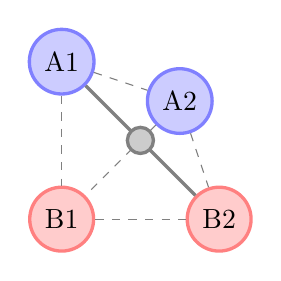
\begin{tikzpicture}[node distance=1cm, auto,]
            \node[very thick, fill=red!20, draw=red!50, circle] (B1) at (0,0) {B1};
            \node[very thick, fill=red!20, draw=red!50, circle] (B2) at (2,0) {B2};
            \node[very thick, fill=blue!20, draw=blue!50, circle] (A1) at (0,2) {A1};
            \node[very thick, fill=blue!20, draw=blue!50, circle] (A2) at (1.5,1.5) {A2};
            \draw[gray, dashed] (A1) -- (B1);
            \draw[gray, very thick] (A1) -- (B2);
            \draw[gray, dashed] (A2) -- (B1);
            \draw[gray, dashed] (A2) -- (B2);
            \draw[gray, dashed] (A1) -- (A2);
            \draw[gray, dashed] (B1) -- (B2);
            \node[very thick, fill=black!20, draw=black!50, circle] (dot) at (1, 1) {};
        \end{tikzpicture}
    \end{subfigure}\begin{subfigure}[b]{0.33\textwidth}
        \centering
        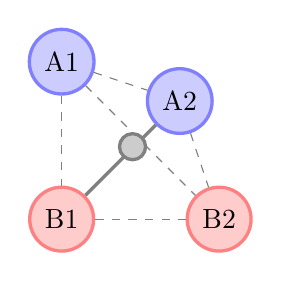
\begin{tikzpicture}[node distance=1cm, auto,]
            \node[very thick, fill=red!20, draw=red!50, circle] (B1) at (0,0) {B1};
            \node[very thick, fill=red!20, draw=red!50, circle] (B2) at (2,0) {B2};
            \node[very thick, fill=blue!20, draw=blue!50, circle] (A1) at (0,2) {A1};
            \node[very thick, fill=blue!20, draw=blue!50, circle] (A2) at (1.5,1.5) {A2};
            \draw[gray, dashed] (A1) -- (B1);
            \draw[gray, dashed] (A1) -- (B2);
            \draw[gray, very thick] (A2) -- (B1);
            \draw[gray, dashed] (A2) -- (B2);
            \draw[gray, dashed] (A1) -- (A2);
            \draw[gray, dashed] (B1) -- (B2);
            \node[very thick, fill=black!20, draw=black!50, circle] (dot) at (0.9, 0.92) {};
        \end{tikzpicture}
    \end{subfigure}\begin{subfigure}[b]{0.33\textwidth}
        \centering
        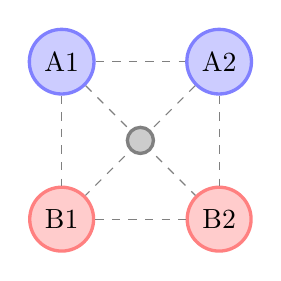
\begin{tikzpicture}[node distance=1cm, auto,]
            \node[very thick, fill=red!20, draw=red!50, circle] (B1) at (0,0) {B1};
            \node[very thick, fill=red!20, draw=red!50, circle] (B2) at (2,0) {B2};
            \node[very thick, fill=blue!20, draw=blue!50, circle] (A1) at (0,2) {A1};
            \node[very thick, fill=blue!20, draw=blue!50, circle] (A2) at (2,2) {A2};
            \draw[gray, dashed] (A1) -- (B1);
            \draw[gray, dashed] (A1) -- (B2);
            \draw[gray, dashed] (A2) -- (B1);
            \draw[gray, dashed] (A2) -- (B2);
            \draw[gray, dashed] (A1) -- (A2);
            \draw[gray, dashed] (B1) -- (B2);
            \node[very thick, fill=black!20, draw=black!50, circle] (dot) at (1, 1) {};
        \end{tikzpicture}
    \end{subfigure}
    \caption{Illustration on why Manifold Mixup learns flatter representations. The interpolation between A1 and B2 in the left panel soft-labels the black dot as 50\% red and 50\% blue, regardless of being very close to a blue point.  
In the middle panel a different interpolation between A2 and B1 soft-labels the same point as ~95\% blue and ~5\% red.  
However, since \emph{Manifold Mixup} \emph{learns} the hidden representations,
    the pressure to predict consistent soft-labels at interpolated points causes the states to become flattened (right panel).}
    \label{fig:intuitive}
\end{figure*}



\section{Manifold Mixup Flattens Representations}
\label{sec:flatten}

We turn to the study of how \manifoldmixup{} impacts the hidden representations of a deep neural network.
At a high level, \manifoldmixup{} flattens the class-specific representations.
More specifically, this flattening reduces the number of directions with significant variance (akin to reducing their number of principal components).

In the sequel, we first prove a theory (Section~\ref{sec:theory}) that characterizes this behavior precisely under idealized conditions. 
Second, we show that this flattening also happens in practice, by performing the SVD of class-specific representations of neural networks trained on real datasets (Section~\ref{sec:empirical}).
Finally, we discuss why the flattening of class-specific representations is a desirable property (Section~\ref{sec:justification}).

\subsection{Theory}
\label{sec:theory}

We start by characterizing how the representations of a neural network are changed by \manifoldmixup{}, under a simplifying set of assumptions.
More concretely, we will show that if one performs mixup in a sufficiently deep hidden layer in a neural network, then the loss can be driven to zero if the dimensionality of that hidden layer  is greater than the number of classes .
As a consequence of this, the resulting representations for that class will have  dimensions.

A more intuitive and less formal version of this argument is given in Figure~\ref{fig:intuitive} and Appendix~\ref{appendix:sec:collision}.  

To this end, assume that  and  denote the input and representation spaces, respectively. We denote the label-set by  and let . Let  denote the set of functions realizable by the neural network, from the input to the representation. Similarly, let  be the set of all functions realizable by the neural network, from the representation to the output.

We are interested in the solution of the following problem in some asymptotic regimes:

More specifically, let  be the empirical distribution defined by a dataset .
Then, let  and  be the minimizers of \eqref{eq:amir:main} for .
Also, let , , and  be a vector space.
These conditions \citep{cybenko1989approximation} state that the mappings realizable by large neural networks are dense in the set of all continuous bounded functions.
In this case, we show that the minimizer  is a linear function from  to .
In this case, the objective \eqref{eq:amir:main} can be rewritten as:

where .
\begin{thm2}
Let  be a vector space of dimension , and let  to represent the number classes contained in some dataset . If , then  and the corresponding minimizer  is a linear function from  to .
\label{thm:mainThm}
\end{thm2}
\begin{proof}
First, we observe that the following statement is true if :

where  and  denote the -dimensional identity matrix and all-one vector, respectively. In fact,  is a rank-one matrix, while the rank of identity matrix is . So,  only needs rank .

Let  for all .
Let  be the -th column of , where  stands for the class-index of the example .
These choices minimize \eqref{eq:amir:main}, since:

The result follows from  for all .
\end{proof}

Furthermore, if , then data points in the representation space  have some degrees of freedom to move independently.
} & \shortstack{Input Mixup\
\max_{g} \min_{d} \mathbb{E}_{x_1,x_2,\lambda,z} \ \ell(d(\text{Mix}_\lambda(x_{1}, x_{2})), y(\lambda; x_{1}, x_{2})),
\label{eq:gan_mixup}

    y(\lambda; x_{1}, x_{2})= 
\begin{cases}
    \lambda,& \text{if } x_{1} \text{ is real and } x_{2} \text{ is fake} \\
    1-\lambda,      & \text{if } x_{1} \text{ is fake and } x_{2} \text{ is real} \\
    0, & \text{if both are fake} \\
    1, & \text{if both are real}
\end{cases}
\label{eq:lambda_cases}

\begin{split}
\max_{g} \min_{d} \mathbb{E}_{x} \ \ell(d(x), 1) + \mathbb{E}_{g(z)} \ \ell(d(g(z)), 0) +
\text{GAN mixup term (Equation \ref{eq:gan_mixup})} 
\end{split}
\label{eq:gan}
\begin{split}
\min_{d} \mathbb{E}_{x_1,x_2,\lambda,z,k} \ \ell(d(x), 1) + \ell(d(g(z), 0) +
\ell(f_{k}(\text{Mix}_\lambda(g_{k}(x_{1}), g_{k}(x_{2}))), y(\lambda; x_{1}, x_{2})),
\end{split}

where  is a function denoting the intermediate output of the discriminator at layer , and  the output of the discriminator given input from layer . 

The layer  we choose the sample can be arbitrary combinations of the input layer (i.e., input mixup), or the first or second resblocks of the discriminator, all with equal probability of selection.

We run some experiments evaluating the quality of generated images on CIFAR10, using as a baseline JSGAN with spectral normalization \citep{spec_norm} (our configuration is almost identical to theirs). Results are averaged over at least three runs\footnote{Inception scores are typically reported with a mean and variance, though this is across multiple splits of samples across a single model. Since we run multiple experiments, we average their respective means and variances.}. From these results, the best-performing mixup experiments (both input and \manifoldmixup{}) is with , with mixing in all layers (both resblocks and input) achieving an average Inception / FID of  / , input mixup achieving 	/ , for the baseline experiment  / . This suggests that mixup acts as a useful regularization on the discriminator, which is even further improved by \manifoldmixup{}. (See Figure \ref{fig:appendix:gan_barplots} for the full set of experimental results.)




\begin{figure}[H]
  \centering
  \includegraphics[width=1.0\linewidth]{figures/chris_gan_test/final.pdf}
  
  \caption{We test out various values of  in conjunction with either: input mixup ( \texttt{pixel}) \citep{zhang2017mixup}, mixing in the output of the first resblock (\texttt{h1}), mixing in either the output  of the first resblock or the output of the second resblock (\texttt{h1,2}), and mixing in the input or the output of the first resblock or the output of the second resblock (\texttt{1,2,pixel}). The dotted line indicates the baseline Inception / FID score. Higher scores are better for Inception, while lower is better for FID.}
  \label{fig:appendix:gan_barplots}
\end{figure}


\section{Intuitive Explanation of how Manifold Mixup avoids Inconsistent Interpolations}
\label{appendix:sec:collision}
An essential motivation behind manifold mixup is that as the network \textit{learns} the hidden states, it does so in a way that encourages them to be a flatter (per-class).  Section~\ref{sec:theory} characterized this for hidden states with any number of dimensions and Figure~\ref{fig:2dbottleneck} showed how this can occur on the 2D spiral dataset.  

Our goal here is to discuss concrete examples to illustrate why this flattening happens, as shown in Figure \ref{fig:intuitive}.  If we consider any two points, the interpolated point between them is based on a sampled  and the soft-target for that interpolated point is the targets interpolated with the same .  So if we consider two points A,B which have the same label, it is apparent that every point on the line between A and B should have that same label with 100\% confidence.  If we consider two points A,B with different labels, then the point which is halfway between them will be given the soft-label of 50\% the label of A and 50\% the label of B (and so on for other  values).  

It is clear that for many arrangements of data points, it is possible for a point in the space to be reached through distinct interpolations between different pairs of examples, and reached with different  values.  Because the learned model tries to capture the distribution , it can only assign a single distribution over the label values to a single particular point (for example it could say that a point is 100\% label A, or it could say that a point is 50\% label A and 50\% label B).  Intuitively, these inconsistent soft-labels at interpolated points can be avoided if the states for each class are more concentrated and the representations do not have variability in directions pointing towards other classes.  This leads to flattening: a reduction in the number of directions with variability.  The theory in Section~\ref{sec:theory} characterizes exactly what this concentration needs to be: that the representations for each class need to lie on a subspace of dimension equal to ``number of hidden dimensions'' - ``number of classes'' + 1.  



\section{Spectral Analysis of Learned Representations}
\label{appendix:sec:flattening}

When we refer to \textit{flattening}, we mean that the class-specific representations have reduced variability in some directions.  Our analysis in this section makes this more concrete.

We trained an MNIST classifier with a hidden state bottleneck in the middle with 12 units (intentionally selected to be just slightly greater than the number of classes).  We then took the representation for each class and computed a singular value decomposition (Figure~\ref{fig:appendix:svd_class_12} and Figure~\ref{fig:appendix:svd_class_30}) and we also computed an SVD over all of the representations together (Figure~\ref{fig:appendix:svd_all}).  Our architecture contained three hidden layers with 1024 units and LeakyReLU activation, followed by a bottleneck representation layer (with either 12 or 30 hidden units), followed by an additional four hidden layers each with 1024 units and LeakyReLU activation.  When we performed \manifoldmixup{} for our analysis, we only performed mixing in the bottleneck layer, and used a beta distribution with an alpha of 2.0.  Additionally we performed another experiment (Figure~\ref{fig:appendix:svd_early_layer} where we placed the bottleneck representation layer with 30 units immediately following the first hidden layer with 1024 units and LeakyReLU activation.  

We found that \manifoldmixup{} had a striking effect on the singular values, with most of the singular values becoming much smaller.  Effectively, this means that the representations for each class have variance in fewer directions.  While our theory in Section~\ref{sec:theory} showed that this flattening must force each classes representations onto a lower-dimensional subspace (and hence an upper bound on the number of singular values) but this explores how this occurs empirically and does not require the number of hidden dimensions to be so small that it can be manually visualized.  In our experiments we tried using 12 hidden units in the bottleneck Figure~\ref{fig:appendix:svd_class_12} as well as 30 hidden units Figure~\ref{fig:appendix:svd_class_30} in the bottleneck.  

Our results from this experiment are unequivocal: \manifoldmixup{} dramatically reduces the size of the smaller singular values for each classes representations.  This indicates a flattening of the class-specific representations.  At the same time, the singular values over all the representations are not changed in a clear way (Figure~\ref{fig:appendix:svd_all}), which suggests that this flattening occurs in directions which are distinct from the directions occupied by representations from other classes, which is the same intuition behind our theory.  Moreover, Figure~\ref{fig:appendix:svd_early_layer} shows that when the mixing is performed earlier in the network, there is still a flattening effect, though it is weaker than in the later layers, and again Input Mixup has an inconsistent effect.  

\begin{figure*}
  \centering
  \includegraphics[width=1.0\linewidth]{figures/singularvalues2.png}
  \caption{SVD on the class-specific representations in a bottleneck layer with 12 units following 3 hidden layers.  For the first singular value, the value (averaged across the plots) is 50.08 for the baseline, 37.17 for Input Mixup, and 43.44 for \manifoldmixup{} (these are the values at x=0 which are cutoff).  We can see that the class-specific SVD leads to singular values which are dramatically more concentrated when using \manifoldmixup{} with Input Mixup not having a consistent effect.  }
  \label{fig:appendix:svd_class_12}
\end{figure*}

\begin{figure*}
  \centering
  \includegraphics[width=1.0\linewidth]{figures/svd_new1.png}
  \caption{SVD on the class-specific representations in a bottleneck layer with 30 units following 3 hidden layers.  For the first singular value, the value (averaged across the plots) is 14.68 for the baseline, 12.49 for Input Mixup, and 14.43 for \manifoldmixup{} (these are the values at x=0 which are cutoff).  }
  \label{fig:appendix:svd_class_30}
\end{figure*}

\begin{figure*}
  \centering
  \includegraphics[width=1.0\linewidth]{figures/svd_early_layer.png}
  \caption{SVD on the class-specific representations in a bottleneck layer with 30 units following a single hidden layer.  For the first singular value, the value (averaged across the plots) is 33.64 for the baseline, 27.60 for Input Mixup, and 24.60 for \manifoldmixup{} (these are the values at x=0 which are cutoff).  We see that with the bottleneck layer placed earlier, the reduction in the singular values from \manifoldmixup{} is smaller but still clearly visible.  This makes sense, as it is not possible for this early layer to be perfectly discriminative.  }
  \label{fig:appendix:svd_early_layer}
\end{figure*}


\begin{figure*}[]
  \centering
  \includegraphics[width=0.7\linewidth,trim={0 0cm 0 0},clip]{figures/svdplots.png}
  \caption{When we run SVD on all of the classes together (in the setup with 12 units in the bottleneck layer following 3 hidden layers), we see no clear difference in the singular values for the Baseline, Input Mixup, and \manifoldmixup{} models.  Thus we can see that the flattening effect of manifold mixup is entirely class-specific, and does not appear overall, which is consistent with what our theory has predicted.  More intuitively, this means that the directions which are being flattened are those directions which point towards the representations of different classes.  }
  \label{fig:appendix:svd_all}
\end{figure*}








\clearpage













 
\end{document}
